\documentclass{article}
\usepackage[utf8]{inputenc}
\usepackage[a4paper, total={6in, 8in}]{geometry}
\usepackage{xcolor,colortbl}
\usepackage{caption}

\title{\LARGE IA-FIB Búsqueda local}
\author{\large Eric Dacal, Joaquim Marset, Josep de Cid}
\date{Marzo 2017}

\usepackage{natbib}
\usepackage{graphicx}

\definecolor{DarkGrey}{HTML}{DFDFDF}
\definecolor{LightGrey}{HTML}{F2F2F2}
\captionsetup[table]{name=Tabla}

\begin{document}

\maketitle

\section{Introducción}

Los algoritmos de búsqueda local son los utilizados en situaciones en que queremos encontrar una solución sin importar el camino para llegar a ella, queriendo siempre alcanzarla en un tiempo razonable, cosa que hace que la óptima sea mayoritariamente inalcanzable. Dada una función heurística que evalúa la calidad de cada solución posible, ésta, guía al algoritmo, que realiza una búsqueda desde una solución inicial mutando a estados solución sucesores, mediante operadores de cambio de estado. Estos algoritmos permiten resolver problemas relacionados con el diseño de redes de distribución, basados el en envío de recursos distribuidos geográficamente en un conjunto de localizaciones que después hacen su distribución o almacenamiento.\par
Nuestro problema consta de un área geográfica de 100km\textsuperscript{2}, en la que se distribuyen un número S de sensores que pueden llegar a capturar 1, 2 o 5 MB/S, y tienen la capacidad de establecer una conexión y transmitir toda la información que tienen almacenada en un mismo instante. Los sensores, sin embargo, tienen ciertas limitaciones, que son tener un máximo de tres conexiones entrantes y no poder transmitir más del triple de información que el mismo puede capturar.\par
Otro elemento del problema, son C centros de datos, que son los destinatarios finales de los datos transmitidos por los sensores. Cada centro de datos puede recibir hasta 150 MB/s, con la limitación de que no puede haber más de 25 conexiones simultáneas.

El objetivo de la práctica es conseguir una configuración en que todos los sensores estén conectados (directa o indirectamente) a un centro de datos, se cumplan las restricciones que presenta cada tipo de nodo, y se maximice la información transmitida a la vez que se minimiza el coste total de la transmisión de la información, de forma que intentemos conectar siempre a sensores más cercanos, o con más ancho de banda para así minimizar costes por distancia a la vez que no perdemos datos por cuellos de botella generados en algunos sensores.\par
En esta práctica analizaremos distintos parámetros para que, tanto con el algoritmo \textit{Hill Climbing} como con el \textit{Simulated Annealing}, dada una función heurística de evaluación que priorice la transmisión máxima de información y unos operadores de cambio de estado con los que generar estados solución sucesores, consigamos encontrar una solución óptima o casi óptima, en un tiempo razonable, de forma que el coste sea lo más pequeño posible y se intente transmitir toda la información.

\newpage
\section{Preguntas}
\begin{enumerate}
  \item \textbf{¿Porqué usamos búsqueda local para resolver este problema?}\par
    En este problema estamos usando búsqueda local porqué tenemos un espacio de búsqueda muy grande. Podemos tener tantas soluciones como las posibles combinaciones que podamos hacer a la hora de decidir a que nodo conectamos un sensor. A causa de este tamaño tan grande, es inabordable encontrar la solución óptima en un tiempo razonable y por eso nos conformamos con una solución que consideremos buena. \par
    Entonces como los algoritmos de búsqueda heurística tienen el objetivo de encontrar el óptimo y en este problema es inviable, usamos búsqueda local para encontrar la mejor solución que podamos.
  \item \textbf{¿Qué elementos intervienen en el problema?}
  \begin{itemize}
      \item \textbf{Sensores:} Son nodos con la capacidad de tanto transmitir como recibir información. Tienen la capacidad de envío de datos limitada a 3 veces la cantidad de información que pueden captar, que puede oscilar entre 1MB/s, 2MB/s o 5MB/s. Tienen las conexiones entrantes limitadas a tres. Se distribuyen aleatoriamente por el mapa dependiendo de la semilla de generación.
      \item \textbf{Centros:} Son nodos con la capacidad de recibir hasta 25 conexiones entrantes, un ancho de banda máximo de 150MB/s y no permiten enviar información ya que son el destino final de esta. Al igual que con los sensores, su distribución también es aleatoria dependiendo de la semilla.
  \end{itemize}
  \item \textbf{¿Cuál es el espacio de búsqueda?}\par
  Todas las posibles soluciones que cumplan las restricción de mantener todos los sensores conectados directa o indirectamente a un centro de datos, sin que ningún nodo supere el máximo de conexiones entrantes permitidas asociadas a su tipo.
  \item \textbf{¿Qué tamaño tiene el espacio de búsqueda?}\par
  Consideramos n como el número de sensores más el número de centros. Teniendo en cuenta la combinatoria de conexiones en que en un nodo hay n posibles entradas, n-1 en la siguiente iteración y así sucesivamente, podemos determinar que el tamaño del espacio de búsqueda es $O$(n!).
  \item \textbf{¿Qué es un estado inicial y que estados iniciales se utilizan?}\par
  Un estado inicial es la primera configuración que comprende una solución válida a partir de la cual se va ejecutar el algoritmo de búsqueda local. Hemos diseñado los siguientes:
   \begin{itemize}
    \item \textbf{Dummy Sequential:} Genera una solución inicial donde cada sensor se conecta con el siguiente sin ordenarlos de ninguna forma, tal y como se genera la lista con la semilla dada, hasta que el último sensor se conecta al centro de datos.
    \item \textbf{Simple Greedy:} Genera una solución inicial ordenando todos los sensores por su capacidad en orden decreciente y siguiendo el orden, conectar cada uno con el primer nodo de mayor capacidad que permita más conexiones (priorizando centros de datos ya que tienen capacidad ilimitada).
    \item \textbf{Distance Greedy:} Al igual que el \textit{Simple Greedy}, genera una solucion ordenando los sensores por capacidad decreciente, y como diferencia, en este se conecta al nodo de mayor capacidad que se encuentre más cerca del sensor.
  \end{itemize}
  Finalmente hemos determinado experimentalmente en posteriores apartados, que el algoritmo que mejor resultados da para nuestros objetivos es el \textit{Distance Greedy}.

  \item \textbf{¿Qué condiciones cumple un estado final?}\par
  En los algoritmos de búsqueda local no existe como tal un estado final ya que son algoritmos que, partiendo de una solución inicial, se aplicarán operadores para ir modificando la solución generando una nueva cada vez, pero no se pueden determinar que condiciones debe cumplir la solución final que generemos ya que dependiendo del algoritmo se puede quedar parado en un punto u otro.\par
  Solo se debe asegurar que con los operadores de cambio de solución, al final de la ejecución del algoritmo, la configuración de la solución sea válida según los criterios del problema. En esta práctica, deberá tener todos los sensores conectados (directa o indirectamente) a uno de los centros de datos.

  \item \textbf{¿Qué operadores permiten modificar los estados?}

  En nuestro caso hemos decidido usar los operadores descritos a continuación ya que partimos de un estado inicial que se encuentra dentro del espacio de soluciones válidas. Por lo tanto para este problema que trata de conexiones entre centros y sensores, no nos interesa operadores como podría ser añadir una conexión o eliminarla ya que siempre partimos de todos los sensores conectados y si desconectamos uno ya nos salimos del espacio de soluciones. Entonces a raíz de esto, para poder movernos dentro del espacio de soluciones, aplicamos los siguientes operadores:

  \begin{itemize}
      \item \textbf{\textit{Swap}:} Dados dos sensores, si la operación no genera un ciclo, intercambia sus conexiones salientes de forma que el primero pasa a estar conectado a la antigua salida del segundo, y viceversa.
      \item \textbf{\textit{Switch}:} Dado un sensor y otro nodo de salida deseado, si los dos sensores no están ya conectados, ni la operación genera un ciclo y el nuevo nodo de salida permite otra conexión entrante, el nuevo nodo pasa a ser el nodo de salida del sensor dado.
  \end{itemize}
  \item \textbf{¿Qué factor de ramificación tienen los operadores de cambio de estado?}\par
  Considerando S el número de sensores y C el número de centros de datos, y que el número de sensores es muy superior al número de centros de datos:
  \begin{itemize}
      \item \textbf{\textit{Swap}:} $O$(s * (s + c)) = $O$(s\textsuperscript{2}).
      \item \textbf{\textit{Switch}:} $O$(s * (s + c)) = $O$(s\textsuperscript{2}).
  \end{itemize}
  \item \textbf{¿Qué factores intervienen en la función heurística? ¿Qué funciones heurísticas habéis escogido?} \par
  Como se ha explicado en la introducción, queremos conseguir una red de conexión donde todos los nodos estén conectados, logremos transmitir la máxima información posible y el menor coste asociado a la red.\par
  Entonces en nuestra función heurística deben aparecer esos dos factores de la información y el coste de la red, maximizando el primero y minimizando el segundo. De esta manera al final lograremos tener una solución que se optimicen estos factores ya que serán los que determinaran la calidad de las soluciones que conformaran nuestro espacio de soluciones.\par
  Esto es debido a que el heurístico guía la búsqueda y en búsqueda local determina lo buena que es una solución. De esta manera cuando se tiene que elegir un sucesor de la solución actual, se elige la solución que da un mejor valor según el heurístico. En nuestro caso una solución será mejor cuando tenga menor coste y transmita más información.\par
  Como debemos tener en cuenta estos dos factores, hemos decidido como función heurística una resta ponderada en la que hemos ponderado con un valor obtenido de forma experimental. De esta forma hemos conseguido que las soluciones envíen el total de la información posible minimizando al máximo el coste ya que con esta ponderación logramos equilibrar los dos factores al ser la información un número tan grande intentando priorizar la información.\par
  Nuestra función heurística es: Coste total de la red - Información transmitida\textsuperscript{2.5} (A causa de que AIMA siempre minimiza a la hora de escoger sucesor).

\end{enumerate}

\newpage
\section{Experimentos}
\begin{enumerate}
  % PREGUNTA 1
  \item \textbf{Determinar qué conjunto de operadores da mejores resultados para una función heurística que optimice el criterio de calidad del problema (3.2) con un escenario en el que el número de centros de datos es 4 y el de sensores es 100. Deberéis usar el algoritmo de Hill Climbing. Escoged una de las estrategias de inicialización de entre las que proponéis. A partir de estos resultados deberéis fijar los operadores para el resto de experimentos. Pensad que con estas proporciones, se podrán transmitir todos los datos.}

  Queremos determinar el conjunto de operadores tales que, partiendo de la solución inicial, nos permitan obtener mejores soluciones al finalizar el algoritmo. En nuestro caso hemos escogido, de las tres maneras de generar la solución inicial, el \textit{Distance Greedy} (ordenamos los sensores de mayor a menor capacidad y cada uno lo conectamos al nodo con más capacidad más próximo a su posición).
  Nuestros posibles operadores son los siguientes:

  \begin{itemize}
    \item \textbf{Switch Operator:} Genera una nueva solución aplicando un cambio de conexión a un sensor concreto. Es decir a uno de los sensores le cambiamos el nodo al que lo conectamos por otro.
    \item \textbf{\textit{Swap} Operator:} Genera una nueva solución aplicando un intercambio de conexiones entre dos sensores. Es decir coge el primer sensor lo desconecta del nodo al que se conectaba y lo conecta al nodo al que se conecta el segundo sensor. De la misma manera se hace con el segundo sensor.
    \item \textbf {Both Operators:} Se hace una combinación de los dos operadores anteriores generando una nueva solución para cada uno.
  \end{itemize}

  Como se ha mencionado al principio, queremos determinar que conjunto de operadores funcionan mejor para una estrategia de generación de solución inicial concreta y una función heurística que optimice los criterios de calidad del problema. En nuestro caso querremos ver cuál de las 3 opciones funcionará mejor.\par
  A priori no podemos saber que opción debemos escoger, por eso el experimento consistirá en partir de una hipótesis donde consideraremos las 3 opciones igual de buenas y hacer 10 réplicas del experimento. Cada réplica se realizará con una semilla aleatoria (una para los centros y otra para los sensores) y para cada posible operador/es de los que disponemos. Así para cada opción se hará bajo las mismas condiciones.\par
  Entonces de cada réplica extraeremos los parámetros que nos servirán para refutar esa hipótesis anteriormente definida. Para este experimento usaremos los que nos definen la calidad de una solución: coste temporal para encontrar la solución, la información transmitida, el coste de la red de conexión y la cantidad de nodos expandidos.

  A modo de resumen el experimento consistirá en:

  \begin{itemize}
  \item \textbf{Observación:}
  Puede haber combinaciones de operadores que den mejores soluciones que otros.
  \item \textbf{Planteamiento:}
  Escogeremos diferentes posibilidades de combinar los operadores y estudiaremos su capacidad para generarnos una solución.
  \item \textbf{Hipótesis:}
   Todas los combinaciones de operadores son igual de buenas a la hora de generar nuevas soluciones (H\textsubscript{0}) o hay algunas mejores que otras (H\textsubscript{1}).
  \item \textbf{Método experimentación:}
    \begin{itemize}
      \item Escogeremos 10 semillas aleatorias (tanto de centros como de sensores), una para cada réplica del experimento.
      \item Para cada réplica ejecutaremos el algoritmo para cada posible opción de combinación de los operadores.
      \item De cada réplica extraeremos parámetros para medir la calidad de la solución y comparar entre las opciones de operadores.
      \item En cada réplica ejecutaremos el algoritmo de Hill Climbing.
      \end{itemize}
  \end{itemize}

  Una vez realizado las réplicas del experimento, hemos obtenido la tabla \ref{table:T1} donde se representa para cada réplica el coste de la red de conexión, las expansiones de nodos sucesores que se producen y el tiempo que tarda el algoritmo en encontrar la solución (no hemos considerado la información transmitida ya que en todas las réplicas, la solución transmite toda la información para cada una de las 3 opciones. Tampoco lo consideraremos en nuestro posterior estudio):

  \begin{figure}[ht]
    \centering
    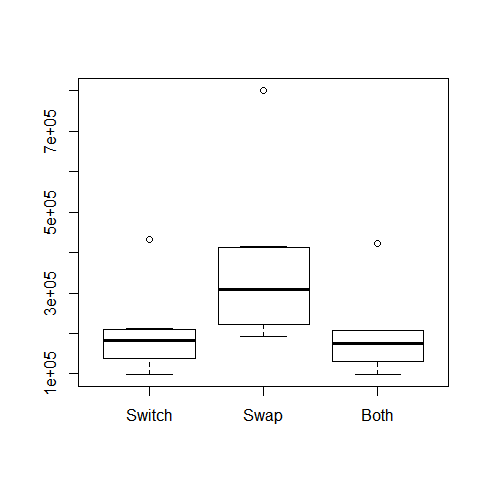
\includegraphics[width=.3\textwidth]{images/operator_Cost_BP}\hfill
    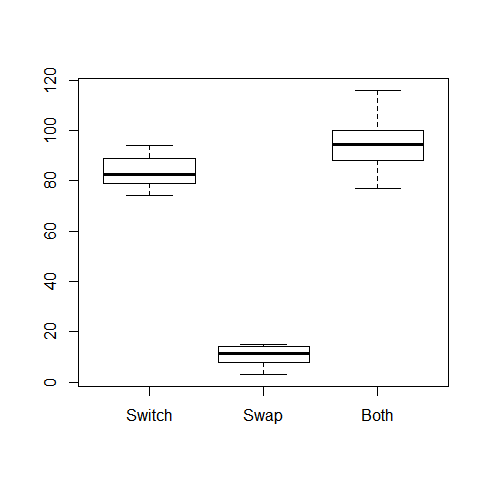
\includegraphics[width=.3\textwidth]{images/operator_Exps_BP}\hfill
    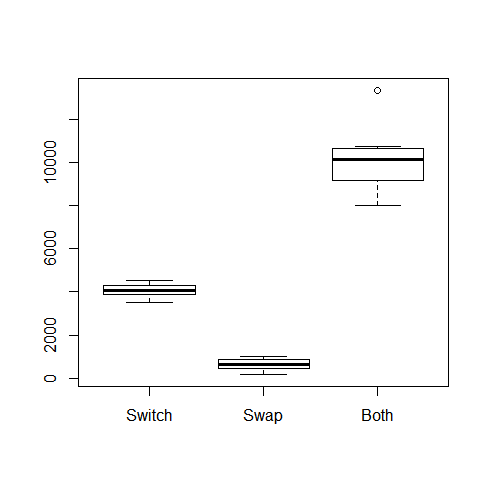
\includegraphics[width=.3\textwidth]{images/operator_Time_BP}
    \caption{Gráficos con los datos de coste, expansiones y tiempo respectivamente}
    \label{fig:BP1}
  \end{figure}

  A partir de los datos de la tabla se han generado los \textit{Boxplot} de la figura \ref{fig:BP1} sobre los cuáles estudiaremos los parámetros que nos evalúan la calidad de la solución para lograr refutar nuestra hipótesis inicial y determinar que conjunto de operadores dan mejor solución. Los \textit{Boxplot}, están representando los costes de la red de conexiones, el tiempo de ejecución y las expansiones que hace \textit{Hill Climbing}. Se observan ciertos valores atípicos causados por la aleatoriedad de la semilla generadora del área geográfica que deja los nodos muy separados entre si y por ello no los consideraremos.

  Ahora que ya hemos presentado los datos obtenidos de las repeticiones del experimento discutiremos esos resultados y llegaremos a la conclusión deseada para este experimento. En este experimento lo haremos comparando los parámetros evaluadores de la calidad de la solución entre pares de las 3 opciones de operadores que hemos definido:

  \begin{itemize}
    \item \textbf{\textit{Switch} Operator - \textit{Swap} Operator:} Como se ve en los resultados, aplicar el operador \textit{Switch} siempre da una mejor solución que solo aplicando el \textit{Swap}. Esto se observa en el coste final de la solución. Respecto a los otros parámetros siempre es menor en el \textit{Swap}, tanto tiempo como expansiones. Esto es debido a que partiendo de nuestra solución inicial, aplicar únicamente el operador \textit{Swap} no permite hacer al algoritmo muchas iteraciones y muy pronto se queda en un máximo local y no continúa. Por eso son tan bajos y no nos permiten hacer una buena comparación de soluciones. Es por eso que solo consideraremos el coste de la red de conexiones. Si miramos los costes vemos que el \textit{Switch} gana en los 10 experimentos. Basándonos en nuestra hipótesis inicial que consideramos como cierta y siguiendo una distribución Binomial con 10 experimentos y una probabilidad de éxito de 0.5 (hemos considerado las dos opciones igual de buenas), la probabilidad que sea éxito en los 10 es de 0.001. Es una probabilidad muy pequeña, significando que es demasiado improbable que pase. Entonces dado que nuestros experimentos son aleatorios significa que contradice nuestra hipótesis inicial y demuestra que aplicar \textit{Switch} es mejor que \textit{Swap}.
    \item \textbf{\textit{Swap} - \textit{Both Operators}:} En este caso ocurre lo mismo que el anterior, solo podemos considerar el coste de la red de conexiones y según nuestros resultados gana la combinación de los dos respecto a usar únicamente \textit{Swap}. De igual forma también, la probabilidad que eso ocurra es muy pequeña si partimos de la misma distribución Binomial provocando que refutemos esa hipótesis inicial y determinemos que es mejor aplicar la combinación de \textit{Switch} y \textit{\textit{Swap}} que solo aplicar \textit{\textit{Swap}}.
    \item \textbf{\textit{Switch} - \textit{Both Operators}:} Finalmente, en esta tercera comparación si que podemos tener en cuenta la mayoría de los parámetros. Entonces si comparamos los costes y siguiendo la misma distribución Binomial que ya venimos usando en las dos comparaciones anteriores, vemos que de los 10 experimentos en los 10 tiene menor coste la combinación de los dos operadores. Por lo tanto en este aspecto vemos que  nuestra H\textsubscript{0} es errónea y aplicar la combinación de los operadores sería mejor. Respecto a los tiempos, nos da que en los 10 experimentos gana siempre aplicar solo \textit{Switch}. Entonces aquí tenemos una contradicción ya que por un lado se refuta la hipótesis inicial determinando que una opción es mejor y por otro lado se determina que es mejor la otra. Entonces debemos considerar que nos interesa más. Si nos fijamos bien, la diferencia de costes entre las dos opciones es bastante pequeña si consideramos que el coste es un número bastante grande. En cambio el tiempo se reduce a la mitad aplicando solo \textit{Switch}. Por tanto teniendo en cuenta que nos interesa también a parte de optimizar los criterios de la solución, encontrar la solución con el menor tiempo determinamos que aplicar solo \textit{Switch} es mejor opción.
  \end{itemize}

  Por tanto como conclusión final uniendo las conclusiones de las tres opciones determinamos que aplicar únicamente el operador de \textit{Switch} como generador de sucesores será la mejor opción para obtener una mejor solución a nuestro problema.

  % PREGUNTA 2
  \item \textbf{Determinar qué estrategia de generación de la solución inicial da mejores resultados para la función heurística usada en el apartado anterior, con el escenario del apartado anterior y usando el algoritmo de Hill Climbing. A partir de estos resultados deberéis fijar también la estrategia de generación de la solución inicial para el resto de experimentos.}

  Un elemento importante en un problema de búsqueda local es la influencia del estado de partida en el coste de la solución final ya que puede decrementar drásticamente el número de pasos al acercarse a la solución óptima. Hemos diseñado las siguientes estrategias de generación de soluciones iniciales:
  \begin{itemize}
    \item \textbf{Dummy Sequential:} Genera una solución inicial donde cada sensor se conecta con el siguiente sin ordenarlos de ninguna forma, tal y como se genera la lista con la semilla dada, hasta que el último sensor se conecta al centro de datos.
    \item \textbf{Simple Greedy:} Genera una solución inicial ordenando todos los sensores por su capacidad en orden decreciente y siguiendo el orden, conectar cada uno con el primer nodo de mayor capacidad que permita más conexiones (priorizando centros de datos ya que tienen capacidad ilimitada).
    \item \textbf{Distance Greedy:} Al igual que el \textit{Simple Greedy}, genera una solución ordenando los sensores por capacidad decreciente, y a diferencia del anterior, en este se conecta al nodo de mayor capacidad que se encuentre más cerca del sensor.
  \end{itemize}

  A priori no podemos determinar si un estado inicial es mejor o peor ya que se desconoce el espacio de búsqueda. Para probar la hipótesis debemos realizar un experimento donde se debe garantizar que cada prueba se realiza en las mismas condiciones. Para ello se han realizado diez réplicas del experimento, donde probamos cada estado inicial descrito, y para ello realizamos cada experimento individual con la misma semilla de números aleatorios para así garantizar que cada prueba tenga una configuración de sensores y centros idéntica en cada uno de los diferentes estados iniciales.\par

  En este caso, la solución de cada experimento no es comparable, ya que cada réplica parte de condiciones distintas, así que debemos tomar otros datos como la calidad de la solución o el tiempo que se tarda en obtenerla, normalmente magnitudes correlacionadas. Con todo esto, el experimento puede ser resumido en los siguientes puntos:
  \begin{itemize}
    \item \textbf{Observación:} Pueden haber estados iniciales que obtienen mejores soluciones que otros.
    \item \textbf{Planteamiento:} Se escogen diversos métodos de generación de estados iniciales y se observan sus soluciones.
    \item \textbf{Hipótesis:} Todos los métodos de inicialización son iguales (H\textsubscript{0}), o hay estados mejores que otros (H\textsubscript{1}).
    \item \textbf{Método experimentación:} \begin{itemize}
        \item Elegir 10 semillas de generación aleatorias, una para cada réplica.
        \item Ejecutar un experimento para cada réplica para la inicialización, con 100 sensores y 4 centros de datos para \textit{Dummy Sequential}, \textit{Simple Greedy} y \textit{Distance Greedy}.
        \item Usar el algoritmo de \textit{Hill Climbing} y medir coste, información, tiempo y nodos expandidos para realizar la comparación.
    \end{itemize}
  \end{itemize}

  Podemos observar los datos generados en cada réplica en la tabla \ref{table:T2}, dónde las estratégias de generación aparecen representadas por sus siglas DS (\textit{Dummy Sequential}), SG (\textit{Simple Greedy}) y DG (\textit{Distance Greedy}):

  \begin{figure}[htp]
    \centering
    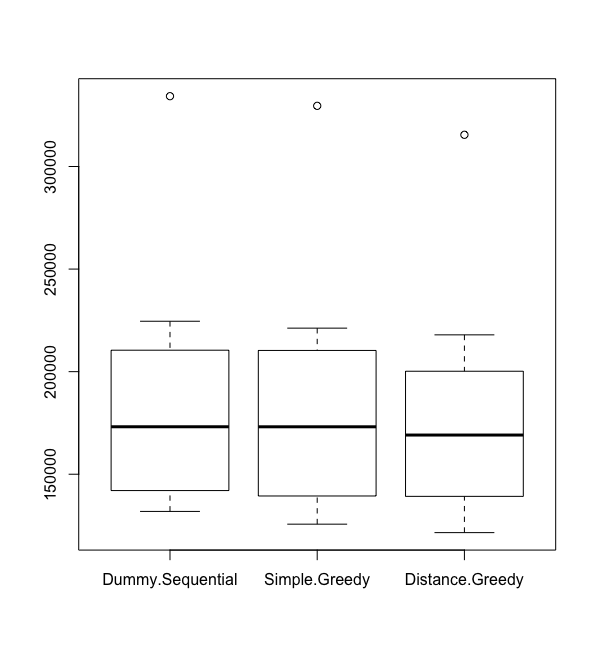
\includegraphics[width=.3\textwidth]{images/initialState_Cost_BP}\hfill
    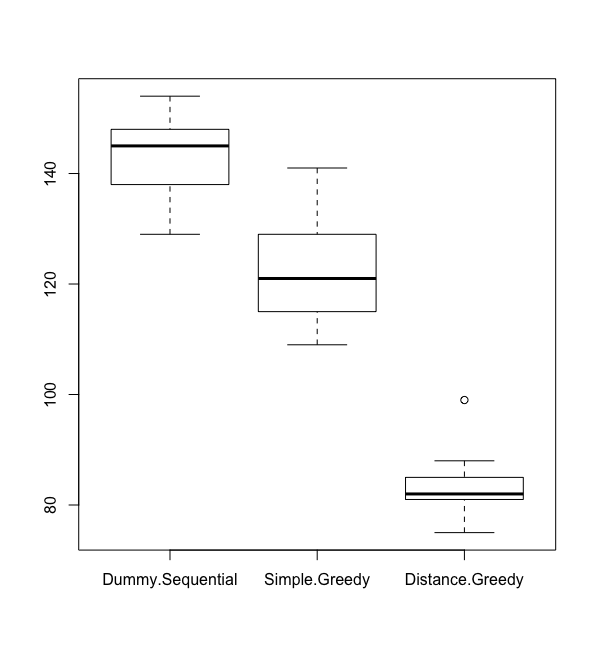
\includegraphics[width=.3\textwidth]{images/initialState_Expansions_BP}\hfill
    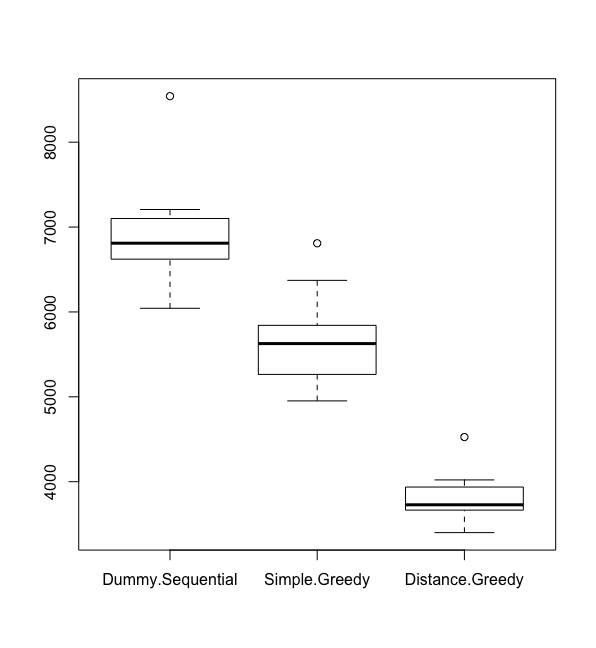
\includegraphics[width=.3\textwidth]{images/initialState_Time_BP}
    \caption{Gráficos con los datos de coste, expansiones y tiempo respectivamente}
    \label{fig:BP2}
  \end{figure}

  A partir de los datos se han generado los \textit{Boxplots} de la figura \ref{fig:BP2}, desde donde vamos a ser analizar los datos y generados y sacar las conclusiones, tratando los datos sin tener en cuenta algunos \textit{outliers} que aparecen con una probabilidad remota debido a la aleatoriedad de los experimentos.\par
  En cuanto a coste final no podemos observar una gran diferencia (ya que está más ligado a los operadores) aunque el \textit{Distance Greedy} consigue una pequeña mejora del coste, con una media de 179835.6, respecto a los 186204.6 del \textit{Dummy Sequential} y los 185195.2 del \textit{Simple Greedy}. Por ello, dejando de lado el coste final que se obtiene, comparamos los resultados por cada pareja de estados iniciales, considerando la probabilidad de que un método de generación de mejores soluciones que los otros para un experimento que se distribuye en forma de función binomial y así comprobamos cual es la probabilidad de que la hipótesis nula sea cierta.

  \begin{itemize}
    \item \textbf{Dummy Sequential - Simple Greedy:} En esta pareja vemos claramente que el \textit{Simple Greedy} da mejores resultados tanto en tiempo como en número de expansiones, por lo que consultamos en la tabla binomial la probabilidad de que en 10 experimentos, el \textit{Simple Greedy} gane en 9 de ellos, suponiendo que las dos estrategias son iguales. Con la resta de las intersecciones [n=10, x=9, p=0.5] y [n=10, x=8, p=0.5] se obtiene que la probabilidad es de 0.0097, por lo que no es cierto que los dos métodos sean iguales, cosa que implica que \textit{Simple Greedy} sea considerado mejor.
    \item \textbf{Dummy Sequential - Distance Greedy:} En este caso se repite el entorno de antes con aún más diferenciada la mejora que presenta el \textit{Distance Greedy}, dando una probabilidad aún más pequeña, de 0.001, así que damos por demostrado que este se considera mejor.
    \item \textbf{Simple Greedy - Distance Greedy:} En este último caso se vuelve a repetir el entorno anterior, con la misma probabilidad de 0.001, por lo que también consideramos como mejor el \textit{Distance Greedy}.
  \end{itemize}

  Cómo conclusión, podemos afirmar que la estrategia de generación \textit{Distance Greedy} es la que genera mejor estado inicial, y es la que se va a usar a partir de ahora en los siguientes experimentos. Aunque en coste está a la par con los otros dos métodos, es claramente mejor en cuestión de tiempo y expansiones, por lo que se puede suponer que la solución inicial generada deja la configuración mucho más cerca de un mínimo.

  %PREGUNTA 3
  \item \textbf{Determinar los parámetros que dan mejor resultado para el Simulated Annealing con el mismo escenario, usando la misma función heurística y los operadores y la estrategia de generación de la solución inicial escogidos en los experimentos anteriores.}

  Para obtener buenos resultados con el algoritmo \textit{Simulated Annealing} es necesario utilizar un número de iteraciones y unos parámetros de aceptación que sean lo más adecuados para el problema planteado, en este caso un escenario de 4 centros de datos con 100 sensores. Para encontrarlos diseñamos el siguiente experimento:

  \begin{itemize}
    \item \textbf{Observación:} Pueden haber valores para los parámetros k y ${\lambda}$ que obtienen mejores soluciones que otros en un mismo escenario.
    \item \textbf{Planteamiento:} Se realiza una búsqueda exhaustiva con diferentes valores de k, de ${\lambda}$ y de las iteraciones totales y entre cambio de temperatura.
    \item \textbf{Hipótesis:} Todos los valores de los parámetros k y ${\lambda}$  producen soluciones igual (H\textsubscript{0}), o hay valores de estos dos parámetros que encuentran mejores soluciones (H\textsubscript{1}).
    \item \textbf{Método experimentación:} \begin{itemize}
        \item Elegir 10 semillas de generación aleatorias, una para cada réplica.
        \item Ejecutar una búsqueda exhaustiva para cada réplica variando los parámetros con los siguiente valores:
        \begin{itemize}
            \item \textbf{Numero de Iteraciones Totales:} Valores entre 1000 y 4000 iteraciones para verificar los mejores parámetros.
            \item \textbf{Numero de Iteraciones entre cambio de temperatura:} Valores entre 100 y 400 iteraciones.
            \item \textbf{Valor de k:} Valores entre 1 y 125.
            \item \textbf{Valor de ${\lambda}$:} Valores entre 0.001 y 1.
        \end{itemize}
        \item Usar el algoritmo de \textit{Simulated Annealing}, medir coste del algoritmo y hacer la media de las diez semillas aleatorias para todas las combinaciones de parámetros.
    \end{itemize}
  \end{itemize}

  \begin{figure}[htp]
    \centering
    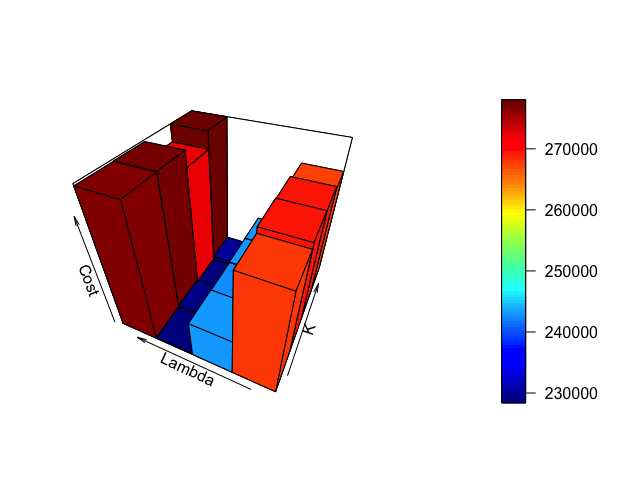
\includegraphics[width=.4\textwidth]{images/parameters_3D}\hfill
    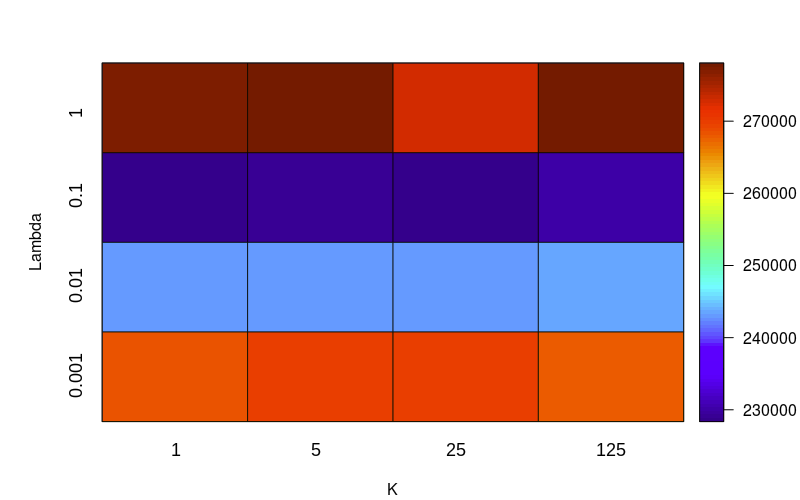
\includegraphics[width=.4\textwidth]{images/parameters_2D}\hfill
    \caption{Variación del coste para los diferentes valores de k y ${\lambda}$}
    \label{fig:CC}
  \end{figure}
  Tras realizar la búsqueda exhaustiva y una vez obtenidos los datos, a partir de estos, se han generado las gráficas de la figura \ref{fig:CC}, podemos observar que hay una relación entre el coste y los parámetros de k y lambda.\par
  La variación de los valores de k parece que no tiene gran relevancia en este problema, aún y así los valores mas óptimos parecen ser los cercanos a 1 y a 125.\par
  La variación de los valores de ${\lambda}$ resulta en cambio mucho mas relevante y se observa que los mejores valores en este problema para ${\lambda}$ son los valores que se encuentra entre 0.001 y 0.1, mientras que los que están por encima o por debajo disminuyen considerablemente la eficiencia en cuanto a coste de las soluciones.\par
  Para analizar la influencia del numero total de iteraciones en el coste obtenido por el algoritmo, vamos a realizar el siguiente problema:

  \begin{itemize}
    \item \textbf{Observación:} El aumento del numero de iteraciones totales produce resultados con menor coste.
    \item \textbf{Planteamiento:} Se realiza una búsqueda exhaustiva con diferentes valores de k, de ${\lambda}$, de las iteraciones totales y de las iteraciones entre cambio de temperatura.
    \item \textbf{Hipótesis:} El numero de iteraciones totales no influye en los costes finales de las soluciones (H\textsubscript{0}), o el numero total de iteraciones disminuye el coste final de las soluciones (H\textsubscript{1}).
    \item \textbf{Método experimentación:} \begin{itemize}
        \item Elegir 10 semillas de generación aleatorias, una para cada réplica.
        \item Ejecutar una búsqueda exhaustiva para cada réplica variando los parámetros con los siguiente valores:
        \begin{itemize}
            \item \textbf{Numero de Iteraciones Totales:} Valores entre 1000 y 10000 iteraciones para verificar los mejores parámetros.
            \item \textbf{Numero de Iteraciones entre cambio de temperatura:} Valores entre 100 y 400 iteraciones.
            \item \textbf{Valor de k:} Valores entre 1 y 125.
            \item \textbf{Valor de ${\lambda}$:} Valores entre 0.001 y 1.
        \end{itemize}
        \item Usar el algoritmo de \textit{Simulated Annealing}, medir coste del algoritmo y hacer la media de las diez semillas aleatorias para todas las combinaciones de parámetros.
    \end{itemize}
  \end{itemize}

 Con estos resultados obtenemos el siguiente gráfico:

  \begin{figure}[htp]
    \centering
    \includegraphics[width=.4\textwidth]{images/Plot_Iterations}\hfill
    \caption{Evolución del coste para diferente numero de iteraciones totales}
    \label{fig:SAPAR}
  \end{figure}

 Dados los siguientes resultados representados en la figura \ref{fig:SAPAR} podemos deducir que el algoritmo obtiene resultados con menor coste al aumentar el numero de iteraciones totales.

 Podemos concluir por tanto que los valores mas óptimos para los parámetros del algoritmo (según nuestro criterio, máximo envío de información con el mínimo coste) \textit{Simulated Annealing} en el caso de un escenario con 100 sensor y con 4 centros de datos, serian:

  \begin{itemize}
    \item \textbf{k} entre 5 y 25.
    \item \textbf{${\lambda}$} con valores cercanos a 0.1.
    \item A mayor numero de iteraciones totales resultados mas óptimo dentro de nuestro criterio.
  \end{itemize}

  \begin{figure}[htp]
    \centering
    \includegraphics[width=.4\textwidth]{images/parameters_HCIncP}\hfill
    \includegraphics[width=.4\textwidth]{images/parameters_SAIncP}\hfill
    \caption{Función del tiempo (ms) respecto al tamaño del problema con ambos algoritmos (rojo \textit{Hill Climbing} y azul \textit{Simulated Annealing}}
    \label{fig:SAHC}
  \end{figure}

  Ya que hemos obtenido los datos para \textit{Simulated Annealing}, también puede resultar interesante ver las diferencias de coste temporal entre este y el algoritmo \textit{Hill Climbing}, para ello creamos los gráficos de la figura \ref{fig:SAHC} que muestran la tendencia de crecimiento que tienen ambos algoritmos. Usamos 10 semillas que irán aumentando gradualmente el numero de centros de 2 en 2 y de sensores de 50 en 50.\par
  Dados estos resultados podemos observar en los gráficos de la figura \ref{fig:SAHC} que el aumento del tamaño del problema produce un aumento temporal en ambos algoritmos.\par
  Los tiempos en \textit{Simulated Annealing} para el mismo tamaño de problema siempre son menores.\par
  En cuanto a la tendencia de crecimiento podemos observar que aunque ambos crecen, aunque el \textit{Simulated Annealing} lo hace con valores muy inferiores al \textit{Hill Climbing}.

  %PREGUNTA 4
  \item \textbf{Dado el escenario de los apartados anteriores, estudiad como evoluciona el tiempo de ejecución para hallar la solución para valores crecientes de los parámetros siguiendo la proporción 4:100. Comenzad con 4 centros de datos e incrementad el número de 2 en 2 hasta que se vea la tendencia. Usad el algoritmo de Hill Climbing y la misma función heurística que antes.}

  De los experimentos anteriores hemos determinado que la mejor estrategia de solución inicial es la de \textit{Distance Greedy} y el mejor operador que podemos aplicar es el \textit{Switch Operator}. Entonces utilizando la función heurística que optimiza los criterios de cualidad de la solución, hemos de ir aumentando los centros de 2 en 2 y los sensores de 50 en 50 de tal manera que manteniendo la proporción de 4:100 podamos ver como afecta en el tiempo de ejecución del algoritmo.

  Sabemos que el tiempo de ejecución del algoritmo es una función que se incrementa respecto el factor de ramificación que tiene cada posible nodo y el tamaño de búsqueda de nuestro problema. Como se ha comentado en el apartado de las preguntas, nuestro espacio de búsqueda tendrá un tamaño factorial respecto el número de centros + sensores y nuestro factor de ramificación será cuadrático respecto los sensores, asintóticamente hablando.

  Realizaremos entonces un conjunto de réplicas del experimento, cambiando la semilla, y para cada réplica haremos una serie de ejecuciones donde en cada una incrementaremos el número de centros y sensores de que disponemos.
  Una vez obtenidos los resultados haremos valores medios para un mismo número de centros y de datos para poder ajustar la función del tiempo, ya que solo para un mismo tamaño el tiempo es comparable.

  El experimento queda resumido de de esta forma:

  \begin{itemize}
    \item \textbf{Observación:} El tiempo sigue una función creciente respecto al número de centros de datos y de sensores que tenemos.
    \item \textbf{Planteamiento:} Partiremos de un número de centros y de sensores e iremos incrementándolos estudiando la variación del tiempo de ejecución
    \item \textbf{Hipótesis:} Incrementando el número de nodos de nuestro problema incrementa el tiempo de ejecución del algoritmo (H\textsubscript{0}), o incrementando el número de nodos no afecta en el tiempo de ejecución (H\textsubscript{1}).
    \item \textbf{Método experimentación:}
    \begin{itemize}
      \item Elegir 10 semillas de generación aleatorias, una para cada réplica.
      \item Para cada réplica ejecutaremos el algoritmo un número de veces donde en cada vez se hará un incremento del número de centros y de sensores manteniendo la proporción 4:100 (cada vez se incrementa en 50 sensores y 2 centros).
      \item Se usará el algoritmo de \textit{Hill Climbing}.
      \item De cada ejecución del algoritmo obtendremos el tiempo de ejecución para luego estudiar como es su variación.
    \end{itemize}
  \end{itemize}

  De cada réplica realizada hemos extraído los tiempos de ejecución de los distintos incrementos de los nodos de nuestra área geográfica y hemos generado la tabla \ref{table:T3} donde en cada columna tenemos el número de sensores y el número de centros. En esta tabla podemos ver como, para cada réplica, evoluciona el tiempo del algoritmo a medida que aumentamos el tamaño de nuestro problema.\par
  Para poder estudiar como es la tendencia de la función de tiempo, consideramos la media de los tiempos, para un mismo número de sensores y centros, de las 10 réplicas y generamos la siguiente gráfica lineal:

  \begin{figure}[ht]
    \centering
    \includegraphics[width=.4\textwidth]{images/increments_TimeP.png}\hfill
    \caption{Evolución del coste temporal al aumentar el número de sensores y centros.}
  \end{figure}

  Como se puede observar en la gráfica, el tiempo de ejecución del algoritmo para encontrar la solución se incrementa a medida que aumentamos el tamaño del problema. Esto es debido a que, al tener más centros y más sensores, tendremos nuevas posibles conexiones entre sensores y centros que podremos establecer.\par
  Entonces al tener más posibilidades de conexión, cada vez que el algoritmo genera todos los sucesores de un nodo, ahora habrá más sucesores para generar y esto se hará por cada iteración que haga el algoritmo hasta que no pueda encontrar una mejor solución. Por lo tanto vemos como al aumentar el factor de ramificación aumenta el coste temporal de la solución.\par
  De la misma forma, al tener más posibles conexiones tenemos nuevas posibles soluciones y por lo tanto nuestro espacio de búsqueda es mayor. Con un mayor espacio de búsqueda el algoritmo puede hacer más iteraciones ya que tiene más soluciones por las que moverse si consiguen mejores resultados referentes a la calidad de la solución. El tener un espacio de soluciones mayor también supone un aumento del coste temporal del algoritmo.\par
  Por lo tanto podemos concluir diciendo que el hecho de aumentar el número de centros de datos y de sensores que tenemos en nuestro problema supondrá un aumento del tiempo de ejecución y este incremento se verá influido por el factor de ramificación de nuestro operador y del tamaño del espacio de búsqueda de nuestro problema.

  %PREGUNTA 5
  \item \textbf{Las proporciones del primer escenario hacen que la capacidad de recibir datos sea mucho mayor que la de captura. A partir de todos los experimentos realizados, ¿hay resultados en los que no todos los centros de datos son utilizados? Si es el caso, estimad la proporción centros de datos/sensores que indican los experimentos.}

  Usando los datos obtenidos en el experimento anterior, en donde se han aumentado los centros:sensores hasta 12:300, se siguen usando la totalidad de los centros de datos, por lo que en todos nuestros experimentos hemos podido observar que el número de centros usados siempre era el máximo, es probable que sea debido a que solo hemos usado operadores de intercambio y además hemos usado un heurístico que prioriza el aumento de la información sobre la disminución del coste.\par
  La definición del heurístico provoca un comportamiento en el algoritmo que produce que siempre se intente enviar la máxima información, consecuentemente siempre se usan el máximo numero de centros de datos en todos los escenarios presentados con anterioridad.\par
  A parte, es improbable que, dada la gran cantidad de sensores y centros que estamos generando aleatoriamente en un mapa relativamente pequeño y finito, haya uno que no tenga ninguna conexión con algún sensor por proximidad


  %PREGUNTA 6
  \item \textbf{Suponiendo que los centros de datos no sean costosos, podríamos estimar como afecta el añadir más centros al coste de la red. Fijando el numero de sensores en 100, realizad experimentos aumentando el número de centros de datos de dos en dos hasta 10 y medid el coste de la red de conexión, el número de centros de datos usados y el coste temporal para hallar la solución. Usad el algoritmo de Hill Climbing y el de Simulated Annealing.}

  Fijando el número de sensores a 100, queremos medir el coste de la red, tiempo utilizado en encontrar la solución y centros de datos usados a medida que incrementamos el número de centros, tanto en \textit{Hill Climbing} como en \textit{Simmulated Annealing}. Vamos a realizar un experimento, resumido a continuación:
  \begin{itemize}
      \item \textbf{Observación:} Incrementar el número de centros de datos manteniendo los mismos sensores puede mejorar el coste del problema.
      \item \textbf{Planteamiento:} Se escogen datos obtenidos con diferente número de centros de datos y se observan los resultados.
      \item \textbf{Hipótesis:} Aumentar el número de centros de datos influye en la solución final (H\textsubscript{0}), o el número de centros de datos no influye en la solución final (H\textsubscript{1}).
      \item \textbf{Método experimentación:}
        \begin{itemize}
            \item Elegir 10 semillas de generación aleatorias, una para cada réplica.
            \item Ejecutar por cada réplica, 4 pruebas, todas con 100 sensores e incrementando los centros de datos de dos en dos en cada una de ellas.
            \item Tanto con el algoritmo de \textit{Hill Climbing} como con el de \textit{Simulated Annealing}, medir coste, tiempo y centros de datos usados.
        \end{itemize}
  \end{itemize}

  \begin{figure}[ht]
    \centering
    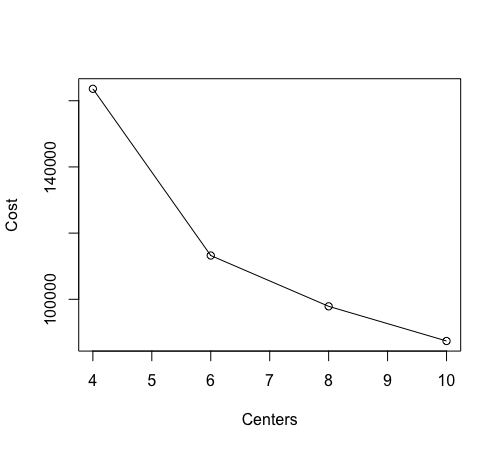
\includegraphics[width=.3\textwidth]{images/dataCenters_Cost_HC_P}\hfill
    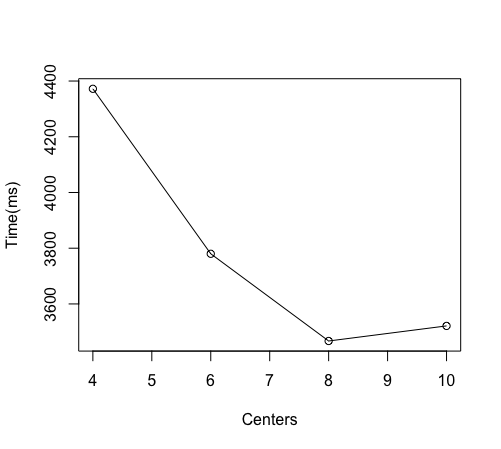
\includegraphics[width=.3\textwidth]{images/dataCenters_Time_HC_P}\hfill
    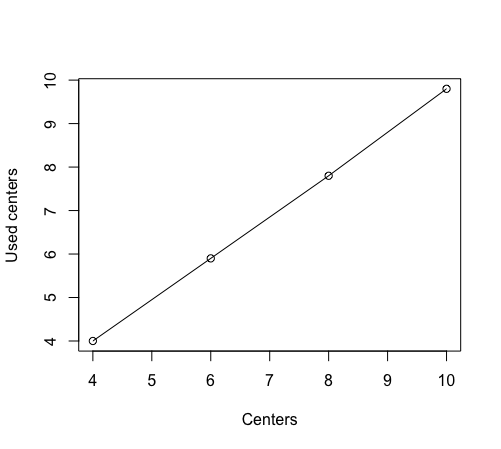
\includegraphics[width=.3\textwidth]{images/dataCenters_Centers_HC_P}
    \caption{Plots con los datos de coste, tiempo y centros usados con el \textit{Hill Climbing}}
    \label{fig:DCCH}
  \end{figure}
  \begin{figure}[ht]
    \centering
    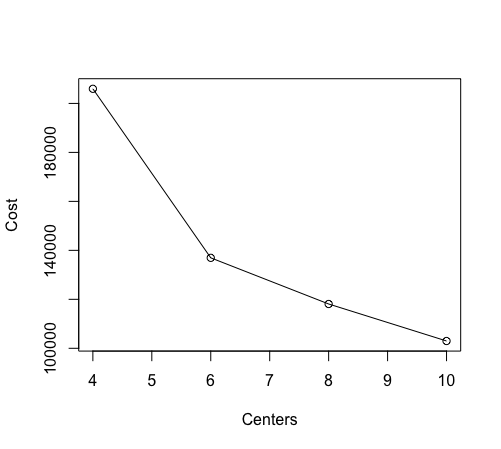
\includegraphics[width=.3\textwidth]{images/dataCenters_Cost_SA_P}\hfill
    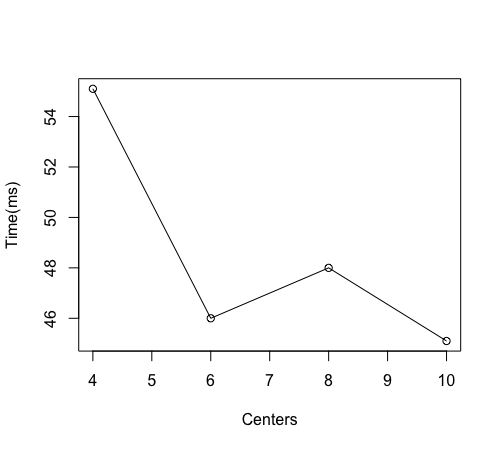
\includegraphics[width=.3\textwidth]{images/dataCenters_Time_SA_P}\hfill
    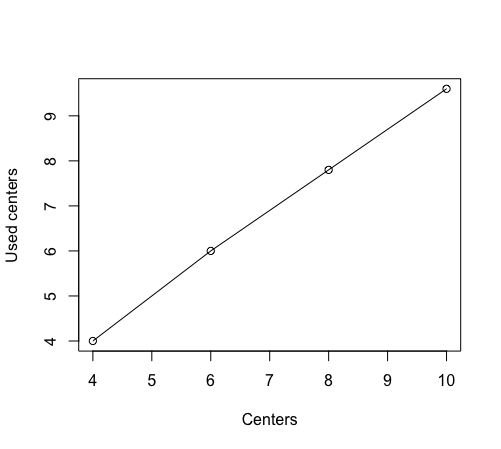
\includegraphics[width=.3\textwidth]{images/dataCenters_Centers_SA_P}
    \caption{Plots con los datos de coste, tiempo y centros usados con el \textit{Simulated Annealing}}
    \label{fig:DCSA}
  \end{figure}

  Con los datos obtenidos de las tablas \ref{table:T4} y \ref{table:T5}, hemos generado los gráficos de las figuras \ref{fig:DCCH} y \ref{fig:DCSA} que muestran la relación centros con coste, tiempo y centros usados respectivamente, tanto con el \textit{Hill Climbing} como con el \textit{Simulated Annealing}.

  Viendo los gráficos, podemos ver la clara influencia del aumento del número de sensores en los tres parámetros que analizamos. Salvo en algunas excepciones de tiempo, que sabiendo que es un parámetro muy variable, puede ser dato por un error de muestreo, vemos que el comportamiento de los dos algoritmos de búsqueda es el mismo.\par
  En cuanto al coste, como más centros de datos hayan más probable es que varios sensores lo consideren como la conexión menos costosa (más cerca) y por lo tanto sea una conexión directa (o con muy pocos sensores intermedios).\par
  En este caso, el tiempo es un parámetro muy ligado al coste ya que creando nuevos centros de datos, al simplificar muchas conexiones el tiempo de cálculo de costes y trasmisión de información, también se ve reducido significativamente.\par
  Con nuestro incremento hasta 10 centros de datos, se puede ver que mayoritariamente todos ellos son usados en al menos una conexión, pero se ve la tendencia de que cada vez puede haber menos que sean usados, ya que por ejemplo, en caso que el número de centros de datos fuese superior al de los sensores, el máximo numero de centros que pueden ser usados a la vez son el número de sensores, dado que cada sensor solo puede estar conectado con un centro.\par
  Como conclusión, podemos afirmar que el número de centros del problema afecta claramente a los parámetros de coste y tiempo, reduciéndolos así de forma significativa. Si tal y como dice el enunciado, consideramos los centros de datos como elementos no costosos, el hecho de añadir el máximo de centros de datos, generará las mejores soluciones.

  %PREGUNTA 7
  \item \textbf{En el escenario que habéis explorado esta prácticamente asegurado el transmitir todos los datos, eso hace que el factor de la función heurística que maximiza los datos transmitidos no tenga casi efecto durante la búsqueda (es constante la mayor parte del tiempo) y que solo se tenga en cuenta el coste de la red de distribución. Ahora cambiaremos el escenario de manera que haya dos centros de datos y 100 sensores. Para buscar soluciones en este escenario, ajustad la función heurística de manera que se puedan dar distintos pesos al factor que mide la cantidad de información enviada. Usad el algoritmo de Hill Climbing en estos experimentos y responded a las siguientes preguntas:}

  Siguiendo la misma estrategia que en los experimentos anteriores, realizando 10 réplicas con semillas aleatorias por cada caso, hemos recogido los datos de coste, información transmitida y tiempo para distintas ponderaciones del heurístico para el valor de la información en la tabla 6, para un peso oscilante entre 1 y 2.8, con iteraciones de 0.2, y con 2.5 para comparar con el resto de experimentos.
  \begin{figure}[ht]
    \centering
    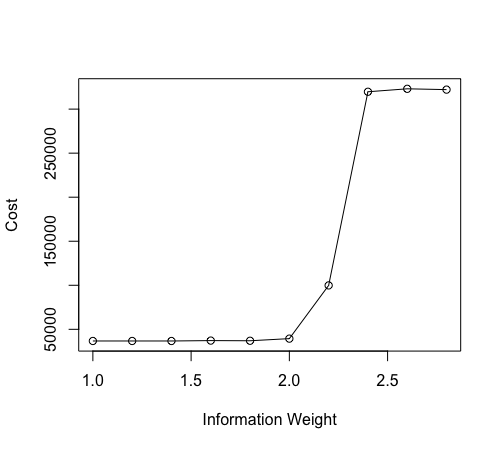
\includegraphics[width=.3\textwidth]{images/heuristic_Cost_P}\hfill
    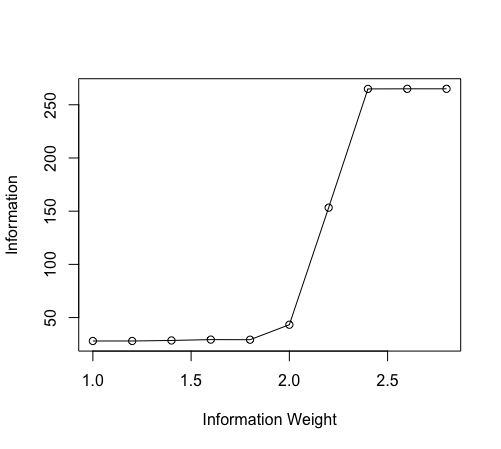
\includegraphics[width=.3\textwidth]{images/heuristic_Information_P}\hfill
    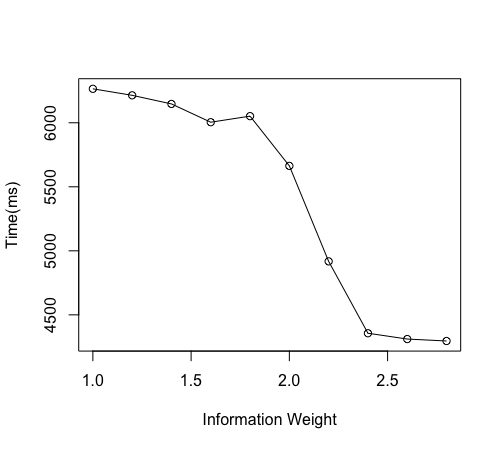
\includegraphics[width=.3\textwidth]{images/heuristic_Time_P}
    \caption{Plots con los datos de coste, tiempo y centros usados con el \textit{Hill Climbing}}
    \label{fig:HP}
  \end{figure}
  \begin{itemize}
    \item \textbf{¿Se ha reducido el tiempo para hallar una solución?}\par
    A medida que aumentamos el peso que asignamos a la información en nuestra función heurística, una resta ponderada, el tiempo se reduce. Esto es debido a que, como vamos nivelando el peso entre el coste y la información transmitida, si el algoritmo encuentra una solución con más información transmitida priorizará la que de más información aunque empeore el coste.\par
    Entonces a la que encuentra una solución donde se transmite toda la información posible ya no hará muchas mas expansiones porqué el heurístico ya no va a permitir elegir como sucesores estados que disminuyen la información transmitida, así que solo va a intentar mejorar el coste. Como es más fácil llegar a transmitir la máxima información, acaba el algoritmo antes.
    \item \textbf{Si usamos una ponderación para el factor que mide la cantidad de información enviada igual que en los primeros escenarios ¿En que proporción aumenta el coste de la red?}\par
    En este experimento hemos reducido el número de centros de datos a la mitad. Como estamos manteniendo la misma función heurística que nos evalúa la calidad, supone pasar a tener el doble de coste. Esto es debido a que al tener menos centros, con nuestra estrategia de solución inicial, los sensores que se conectaban a los dos centros de más que teníamos ahora se conectarán a un sensor con la mejor capacidad posible. Entonces como el coste se calcula como distancia por información transmitida a cada uno de los dos centros que tenemos ahora tendrá más sensores que se conectarán a él indirectamente. Por tanto será mas información que le llegará y eso supondrá mayor coste. \par
    Para ver los resultados dados por nuestros experimentos dividimos la media del coste generado con 2 y 4 centros respectivamente, ambos con la misma ponderación usada en el resto de los experimentos (2.5) que nos da una proporción de aumento de coste de 1.906395.
    \item \textbf{¿Cómo cambia el coste de la red en función de la ponderación que se da al envío de los datos? ¿Hay una ponderación a partir de la que el coste de la red ya no aumenta?}\par
    Observando la figura \ref{fig:HP}, podemos ver que el coste y la información están correlaciones en cuanto al peso de la información se refiere. Eso es algo coherente ya que si el heurístico prioriza la información no le va a dar casi nada de importancia al coste y en general este tenderá a empeorar a cambio de incrementar la información transmitida, hasta que a partir de cierta ponderación obtengamos la información máxima que se puede transmitir, y el algoritmo pase a intentar optimizar el coste.\par
    En nuestro caso con 100 sensores y 2 centros de datos, aproximadamente a partir de una ponderación de 2.5, obtenemos el máximo de información que puede transmitir dicha configuración (265MB/s) por lo que el coste va a dejar de aumentar, ya que la información no puede ser mejorada y lo único que reduce el heurístico será intentar disminuir el coste.
  \end{itemize}

  %PREGUNTA 8
  \item \textbf {Experimento Especial: Para fomentar el trabajo continuado en la practica siguiendo la planificación, asignaremos un punto extra sobre la nota de la práctica a los grupos que envíen durante la semana del 20 al 25 de marzo un correo con el resultado del coste total de transmisión que se obtiene en el escenario con 4 centros de datos y 100 sensores y cuánto tiempo se tarda en hallar la solución en milisegundos (aproximadamente). Para que todos los experimentos sean con las mismas condiciones usaremos como semilla del generador de números aleatorios 1234, para generar los centros y sensores. Deberéis usar los operadores, inicialización y heurística escogidos con los experimentos 1 y 2. Los grupos que manden el correo, tendrán que enseñar la ejecución de la práctica con este escenario al profesor de laboratorio durante las sesiones de laboratorio de la semana siguiente. Obviamente ha de dar el mismo resultado.}

  Para este experimento hemos usado el algoritmo \textit{Hill Climbing} indicado en el enunciado. Teniendo en cuenta los resultados de los experimentos 1 y 2 hemos escogido como único operador \textit{Switch} y como solución inicial \textit{Distance Greedy} ya que hemos visto que son los que generaban mejores resultados. Tal y como se describe en el enunciado hemos usado un escenario con 4 centros de datos y 100 sensores y hemos usado la semilla generadora 1234. Hemos obtenido en nuestra ejecución los siguientes resultados:
  \begin{itemize}
    \item \textbf{Coste Total:} 260734.0
    \item \textbf{Información Total:} 265.0
    \item \textbf{Tiempo Total:} 11.606ms
  \end{itemize}
  \end{enumerate}

\newpage
\section{Trabajo de innovación}
 El tema que hemos elegido para el trabajo de innovación es la Inteligencia Artificial desarrollado por \textit{Google DeepMind} para jugar al juego Go,  un juego de tablero estratégico para dos jugadores similar al ajedrez, pero con mucha complejidad añadida. Conocida como \textbf{AlphaGo} se convirtió a finales del 2015 en la primera IA capaz de ganar a un jugador profesional de Go sin \textit{handicap} en un tablero de 19x19. \textbf{AlphaGo} usa un árbol de búsqueda de Monte Carlo, que encuentra los movimientos a realizar basado en un aprendizaje automático realizado previamente, usando una red neuronal artificial, un método de \textit{Deep Learning}.
  La repartición se va a generar de la siguiente forma:
 \begin{itemize}
     \item \textbf{Josep de Cid:} Identificar las innovaciones de la empresa basadas en técnicas y métodos de la inteligencia artificial.
     \item \textbf{Eric Dacal:} Analizar riesgos y beneficios de dicha innovación para la empresa.
     \item \textbf{Joaquim Marset:} Tener en cuenta a quien afecta la innovación y de que forma lo hace (riesgos y beneficios).
 \end{itemize}
 Referencias:
 \begin{itemize}
     \item [24-3] https://deepmind.com/research/alphago/
     \item [24-3] http://www.lavanguardia.com/vida/20160312/40383449463/google-go-alpha-go-lee-sedol.html
     \item [24-3] https://es.wikipedia.org/wiki/AlphaGo
     \item [31-3] https://gogameguru.com/i/2016/03/deepmind-mastering-go.pdf
     \item [31-3] https://www.wired.com/2016/05/google-alpha-go-ai/
     \item [31-3] https://journals.aps.org/prl/abstract/10.1103/PhysRevLett.71.211
     \item [1-4] http://www.theprojectspot.com/tutorial-post/introduction-to-artificial-neural-networks-part-1/7
     \item [1-4] http://es.gizmodo.com/la-victoria-de-alphago-ha-infundido-miedo-a-la-intelige-1765225056
     \item [1-4]http://homepages.cwi.nl/~aeb/go/games/games/AlphaGo/
     \item [2-4] https://www.wired.com/2016/01/googles-go-victory-is-just-a-glimpse-of-how-powerful-ai-will-be/
 \end{itemize}
 Aunque el código de \textbf{AlphaGo} no es \textit{OpenSource}, al ser un programa desarrollado por Google, y que tuvo un gran impacto al ser la primera máquina capaz de lograr una victoria en esas condiciones, existen numerosos recursos respecto a las técnicas que usa, algoritmos de búsqueda, configuración y rendimiento de la máquina...

\newpage
\section{Apéndice}
  \begin{center}
    \begin{tabular}{ | r | r | r | r | r | r | r | r | r | r | }
      \hline
      \rowcolor{DarkGrey}
      & \multicolumn{3}{|c|}{Coste} & \multicolumn{3}{c|}{Expansiones} & \multicolumn{3}{|c|}{Tiempo\textsubscript{ms}} \\ \hline
      \rowcolor{DarkGrey}
      \multicolumn{1}{|c|}{Réplica} & \multicolumn{1}{|c|}{Switch} & \multicolumn{1}{|c|}{Swap} & \multicolumn{1}{|c|}{Both} & \multicolumn{1}{|c|}{Switch} & \multicolumn{1}{|c|}{Swap} & \multicolumn{1}{|c|}{Both} & \multicolumn{1}{|c|}{Switch} & \multicolumn{1}{|c|}{Swap} & \multicolumn{1}{|c|}{Both} \\ \hline \hline
      1 & 138820 & 221734 & 130076 & 79 & 13 & 96 & 4398 & 865 & 10148 \\ \hline
      \rowcolor{LightGrey}
      2 & 163489 & 272548 & 157841 & 82 & 3 & 92 & 3920 & 167 & 9460 \\ \hline
      3 & 212074 & 405524 & 206322 & 89 & 14 & 98 & 4294 & 787 & 10083 \\ \hline
      \rowcolor{LightGrey}
      4 & 174042 & 415124 & 184906 & 74 & 4 & 88 & 3512 & 212 & 9174 \\ \hline
      5 & 191924 & 210339 & 217941 & 94 & 11 & 100 & 4511 & 625 & 10620 \\ \hline
      \rowcolor{LightGrey}
      6 & 98688.0 & 193339 & 98140 & 81 & 12 & 83 & 3883 & 671 & 8684 \\ \hline
      7 & 431491 & 802128 & 423005 & 90 & 14 & 116 & 4167 & 928 & 13342 \\ \hline
      \rowcolor{LightGrey}
      8 & 115756 & 195480 & 113964 & 76 & 9 & 77 & 3906 & 575 & 7996 \\ \hline
      9 & 210121 & 411938 & 207363 & 89 & 8 & 101 & 4194 & 455 & 10721 \\ \hline
      \rowcolor{LightGrey}
      10 & 206091 & 314234 & 204089.0 & 83 & 15 & 93 & 3897 & 1006 & 10565 \\ \hline
    \end{tabular}
    \captionof{table}{Tabla con el coste, expansiones y tiempo de cada operador.}
    \label{table:T1}
  \end{center}

  \begin{center}
    \begin{tabular}{ | r | r | r | r | r | r | r | r | r | r | }
      \hline
      \rowcolor{DarkGrey}
      & \multicolumn{3}{|c|}{Coste} & \multicolumn{3}{c|}{Expansiones} & \multicolumn{3}{|c|}{Tiempo\textsubscript{ms}} \\ \hline
      \rowcolor{DarkGrey}
      \multicolumn{1}{|c|}{Réplica} & \multicolumn{1}{|c|}{DS} & \multicolumn{1}{|c|}{SG} & \multicolumn{1}{|c|}{DG} & \multicolumn{1}{|c|}{DS} & \multicolumn{1}{|c|}{SG} & \multicolumn{1}{|c|}{DG} & \multicolumn{1}{|c|}{DS} & \multicolumn{1}{|c|}{SG} & \multicolumn{1}{|c|}{DG} \\ \hline \hline
      1 & 131871 & 125657 & 121535 & 145 & 129 & 88 & 8542 & 5842 & 4021 \\ \hline
      \rowcolor{LightGrey}
      2 & 192921 & 192636 & 184075 & 148 & 115 & 83 & 7039 & 5278 & 3728 \\ \hline
      3 & 146387 & 148113 & 144927 & 146 & 115 & 79 & 6888 & 5264 & 3529 \\ \hline
      \rowcolor{LightGrey}
      4 & 142036 & 138780 & 139212 & 154 & 129 & 81 & 7207 & 5805 & 3728 \\ \hline
      5 & 224573 & 210339 & 217941 & 145 & 123 & 75 & 6732 & 5563 & 3400 \\ \hline
      \rowcolor{LightGrey}
      6 & 334282 & 329574 & 315465 & 129 & 119 & 99 & 6190 & 5691 & 4526 \\ \hline
      7 & 210457 & 221211 & 200202 & 139 & 109 & 81 & 6680 & 4952 & 3743 \\ \hline
      \rowcolor{LightGrey}
      8 & 163742 & 169532 & 161120 & 130 & 141 & 81 & 6043 & 6809 & 3701 \\ \hline
      9 & 133242 & 139395 & 136800 & 149 & 113 & 83 & 7101 & 5165 & 3665 \\ \hline
      \rowcolor{LightGrey}
      10 & 182535 & 176715 & 177079 & 138 & 136 & 85 & 6622 & 6372 & 3937 \\ \hline
    \end{tabular}
    \captionof{table}{Tabla con el coste, expansiones y tiempo de cada estado inicial.}
    \label{table:T2}
  \end{center}

  \begin{center}
    \begin{tabular}{ | r | r | r | r | r | r | }
      \hline
      \rowcolor{DarkGrey}
      & \multicolumn{5}{|c|}{Tiempo\textsubscript{ms}} \\ \hline
      \rowcolor{DarkGrey}
      \multicolumn{1}{|c|}{Réplica} & \multicolumn{1}{|c|}{100-4} & \multicolumn{1}{|c|}{150-6} & \multicolumn{1}{|c|}{200-8}
      & \multicolumn{1}{|c|}{250-10} & \multicolumn{1}{|c|}{300-12}\\ \hline \hline
      1 & 4322 & 18280 & 137359 & 541277 & 1013316 \\ \hline
      \rowcolor{LightGrey}
      2 & 4044 & 20226 & 135236 & 513573 & 856172 \\ \hline
      3 & 4157 & 21828 & 159616 & 663291 & 998188 \\ \hline
      \rowcolor{LightGrey}
      4 & 3989 & 19824 & 131874 & 550534 & 974540 \\ \hline
      5 & 4394 & 22133 & 168454 & 582814 & 991376 \\ \hline
      \rowcolor{LightGrey}
      6 & 4292 & 19782 & 160546 & 499572 & 907507 \\ \hline
      7 & 4798 & 21657 & 173795 & 589602 & 937619  \\ \hline
      \rowcolor{LightGrey}
      8 & 4352 & 20604 & 152151 & 545123 & 1126427 \\ \hline
      9 & 4190 & 19980 & 150642 & 676311 & 974686 \\ \hline
      \rowcolor{LightGrey}
      10 & 4280 & 18739 & 169196 & 539027 & 948189\\ \hline
    \end{tabular}
    \captionof{table}{Tabla con el coste temporal al ir incrementando los sensores y los centros siguiendo la proporción 4:100.}
    \label{table:T3}
  \end{center}

  \begin{center}
    \begin{tabular}{ | r | r | r | r | r | r | r | r | r | r | r | r | r | }
      \hline
      \rowcolor{DarkGrey}
      & \multicolumn{3}{|c|}{4 Centros} & \multicolumn{3}{c|}{6 Centros} & \multicolumn{3}{|c|}{8 Centros} & \multicolumn{3}{|c|}{10 Centros} \\ \hline
      \rowcolor{DarkGrey}
      \multicolumn{1}{|c|}{Réplica} & \multicolumn{1}{|c|}{C} & \multicolumn{1}{|c|}{T} & \multicolumn{1}{|c|}{CU} & \multicolumn{1}{|c|}{C} & \multicolumn{1}{|c|}{T} & \multicolumn{1}{|c|}{CU} & \multicolumn{1}{|c|}{C} & \multicolumn{1}{|c|}{T} & \multicolumn{1}{|c|}{CU} & \multicolumn{1}{|c|}{C} & \multicolumn{1}{|c|}{T} & \multicolumn{1}{|c|}{CU} \\ \hline \hline
      1 & 141143 & 5436 & 4 & 116345 & 4033 & 6 & 101003 & 3504 & 8 & 79442 & 3303 & 10 \\ \hline
      \rowcolor{LightGrey}
      2 & 156574 & 4669 & 4 & 121075 & 3957 & 6 & 115976 & 3981 & 7 & 113936 & 3980 & 9 \\ \hline
      3 & 219954 & 4073 & 4 & 150877 & 4028 & 6 & 145484 & 3704 & 8 & 105131 & 3995 & 10 \\ \hline
      \rowcolor{LightGrey}
      4 & 199729 & 4353 & 4 & 159968 & 4119 & 5 & 149226 & 3519 & 7 & 138371 & 4335 & 9\\ \hline
      5 & 158359 & 4012 & 4 & 111928 & 3862 & 6 & 99208 & 3207 & 8 & 93913 & 3129 & 10\\ \hline
      \rowcolor{LightGrey}
      6 & 135497 & 3841 & 4 & 102283 & 3186 & 6 & 65554 & 3353 & 8 & 59739 & 3729 & 10  \\ \hline
      7 & 150857 & 4299 & 4 & 109235 & 3857 & 6 & 73672 & 2862 & 8 & 64206 & 3072 & 10  \\ \hline
      \rowcolor{LightGrey}
      8 & 125284 & 4310 & 4 & 73048 & 3250 & 6 & 75328 & 3976 & 8 & 66731 & 3336 & 10  \\ \hline
      9 & 206598 & 4541 & 4 & 74990 & 3726 & 6 & 70653 & 3181 & 8 & 71507 & 3242 & 10 \\ \hline
      \rowcolor{LightGrey}
      10 & 142046 & 4187 & 4 & 112513 & 3782 & 6 & 82646 & 3383 & 8 & 81054 & 3090 & 10 \\ \hline
    \end{tabular}
    \captionof{table}{Tabla con el coste C, tiempo T y centros usados CU incrementando el número de centros para \textit{Hill Climbing}.}
    \label{table:T4}
  \end{center}

  \begin{center}
    \begin{tabular}{ | r | r | r | r | r | r | r | r | r | r | r | r | r | }
      \hline
      \rowcolor{DarkGrey}
      & \multicolumn{3}{|c|}{4 Centros} & \multicolumn{3}{c|}{6 Centros} & \multicolumn{3}{|c|}{8 Centros} & \multicolumn{3}{|c|}{10 Centros} \\ \hline
      \rowcolor{DarkGrey}
      \multicolumn{1}{|c|}{Réplica} & \multicolumn{1}{|c|}{C} & \multicolumn{1}{|c|}{T} & \multicolumn{1}{|c|}{CU} & \multicolumn{1}{|c|}{C} & \multicolumn{1}{|c|}{T} & \multicolumn{1}{|c|}{CU} & \multicolumn{1}{|c|}{C} & \multicolumn{1}{|c|}{T} & \multicolumn{1}{|c|}{CU} & \multicolumn{1}{|c|}{C} & \multicolumn{1}{|c|}{T} & \multicolumn{1}{|c|}{CU} \\ \hline \hline
      1 & 150572 & 90 & 4 & 131439 & 49 & 6 & 145241 & 46 & 8 & 102257 & 46 & 10 \\ \hline
      \rowcolor{LightGrey}
      2 & 197279 & 50 & 4 & 157840 & 47 & 6 & 128963 & 79 & 8 & 120325 & 45 & 8 \\ \hline
      3 & 265559 & 49 & 4 & 163995 & 46 & 6 & 166553 & 46 & 6 & 120207 & 49 & 10 \\ \hline
      \rowcolor{LightGrey}
      4 & 219923 & 47 & 4 & 186936 & 45 & 6 & 167751 & 44 & 8 & 170368 & 44 & 9\\ \hline
      5 & 209098 & 47 & 4 & 127356 & 45 & 6 & 160074 & 45 & 8 & 100144 & 44 & 10 \\ \hline
      \rowcolor{LightGrey}
      6 & 165657 & 47 & 4 & 115875 & 45 & 6 & 72280 & 44 & 8 & 90211 & 44 & 9 \\ \hline
      7 & 167286 & 48 & 4 & 136600 & 46 & 6 & 77000 & 44 & 8 & 67110 & 45 & 10 \\ \hline
      \rowcolor{LightGrey}
      8 & 249886 & 49 & 4 & 121356 & 46 & 6 & 78563 & 44 & 8 & 76002 & 46 & 10 \\ \hline
      9 & 228870 & 76 & 4 & 106391 & 45 & 6 & 71225 & 43 & 8 & 98142 & 44 & 10 \\ \hline
      \rowcolor{LightGrey}
      10 & 205535 & 48 & 4 & 121626 & 46 & 6 & 113284 & 45 & 8 & 85056 & 44 & 10\\ \hline
    \end{tabular}
    \captionof{table}{Tabla con el coste (C), tiempo (T\textsubscript{ms}) y centros usados (CU) incrementando el número de centros para \textit{Simulated Annealing}.}
    \label{table:T5}
  \end{center}

    \begin{center}
    \begin{tabular}{ | r | r | r | r | }
      \hline
      \rowcolor{DarkGrey}
      \multicolumn{1}{|c|}{Peso información} & \multicolumn{1}{|c|}{Coste} & \multicolumn{1}{|c|}{Información} & \multicolumn{1}{|c|}{Tiempo\textsubscript{ms}} \\ \hline \hline
      1 & 36755.1 & 28.0 & 6265.2 \\ \hline
      \rowcolor{LightGrey}
      1.2 & 36755.5 & 28.0 & 6214.3 \\ \hline
      1.4 & 36744.4 & 28.5 & 6147.3 \\ \hline
      \rowcolor{LightGrey}
      1.6 & 37198.0 & 29.3 & 6004.4 \\ \hline
      1.8 & 37006.3 & 29.2 & 6051.8 \\ \hline
      \rowcolor{LightGrey}
      2.0 & 39430.8 & 43.3 & 5663.3 \\ \hline
      2.2 & 99856.1 & 155.3 & 4917.6 \\ \hline
      \rowcolor{LightGrey}
      2.4 & 319702.6 & 264.9 & 4356.4 \\ \hline
      2.5 & 324316.5 & 265.0 & 4325.2 \\ \hline
      \rowcolor{LightGrey}
      2.6 & 323055.3 & 265.0 & 4311.0 \\ \hline
      2.8 & 322132.1 & 265.0 & 4295.8 \\ \hline
    \end{tabular}
    \captionof{table}{Tabla con el coste, información transmitida y tiempo medio incrementando el peso de la información en el heurístico para \textit{Hill Climbing}.}
    \label{table:T7}
  \end{center}

\end{document}